

The purpose of the thesis was to increase the conversion rate of an e-commerce search application 
by providing more relevant search results. 
While the earlier chapter provided the necessary background information, the purpose
of this chapter is to introduce the current search application and how it works
from receiving the query from the customer to providing the search results back to the customer. 


In addition, the chapter introduces the process of managing 
the search ranking and monitoring the current search application.
The conclusions in this chapter are based on a survey about the status of the current search \cite{searchSurvey}.
The survey was also answered by the managers of the current search application responsible for keeping
the search ranking up-to-date.
The survey also collected the ideas on how the current setup could be improved and 
what is useful in the current setup.


\section{Performing query and receiving results}

The current search application is on multiple websites of the organization across the Nordic countries. 
There is one back-end that handles all traffic and multiple Elasticsearch clusters for each website to 
hold the website specific data. Figure \ref{fig:current-solution} describes the application
from the input of the customer to the customer receiving the search results back.
The areas related to this thesis highlighted in red.

\begin{figure}
    \centering
    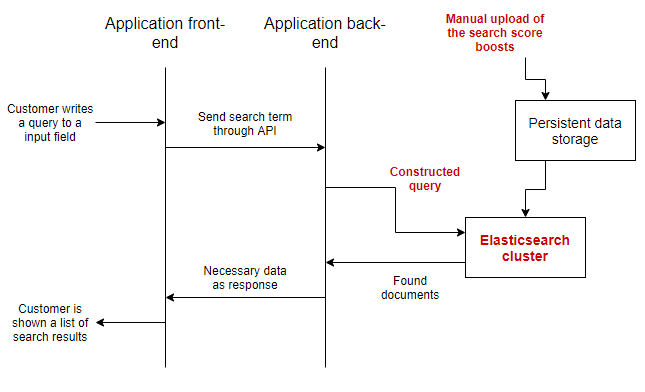
\includegraphics[width=\textwidth]{img/current-solution.png}
    \caption{Diagram of the current search application with targeted areas highlighted in red.}
    \label{fig:current-solution}
\end{figure}

While the implementation required some work in the front-end of the application to enable A/B testing, 
there is no need to go into detail how the application works other than the affected elements.
The application front-end uses an HTTP request to communicate the input query to the back-end application, 
which constructs a query from the input.
Then, the constructed query is sent to Elasticsearch cluster through the Query API, which returns a set of documents
matching to the query which again is enriched with necessary data and sent back to the front-end to show the results
to the customer.


Elasticsearch is a powerful tool when it comes to searching, in addition to providing many  
tools to make efficient queries to show relevant results to customers.
However, the current search application has not been developed much in the last few years 
due to other projects taking priority over it. 
Therefore, it is missing out on some of the powerful tools provided by Elasticsearch.
In addition to the implementation being outdated, 
it lacks automation in the business score calculation for the products.


The current solution indexes documents in an inefficient manner. 
While indexing a document in Elasticsearch is very fast, it still requires quite a lot of computing 
power when indexing thousands of documents at the same time. 
The current search application utilizes only one analyzer, the language analyzer, in one field only.
Furthermore, it contradicts with the function that creates the index for the product data, since it has
multiple analyzers defined for multiple fields which are not utilized at all.
These analyzers are most likely left there from some previous implementation.


The application utilizes a wildcard search, which adds wildcard terms to both
the start and the end of each search term in the query, as seen in Figure \ref{fig:current-query}.
In some cases, the wildcards in both ends of the search term make sense but may produce 
inaccurate search results when search terms are short.
For instance, the results for a query ``tv`` might be confusing since two letters might match 
many terms in the inverted index when used with wildcards.
In summary, the lack of text analysis used, and the lack of effort put into constructing the query is 
correlated with the lack of effort that has been put to developing the search application.


The problems with the current search application can be seen in the query shown in Figure \ref{fig:current-query}.
The query object shows that the query is searched across multiple fields, 
and the fields have separate boosts defined to them. 
For instance, \emph{title\textasciicircum15} in the query means that the content score calculated for the term matching to the title field
should be multiplied by 15.
Elasticsearch, by default, matches to the best field only, 
the field with the highest content score.
Consequently, boosting a field makes it more likely to be the best field if a match is found from it.
It makes sense that a match found from the title of the product should be prioritized over
a match in, for instance, sales arguments, it is difficult to say by how much it should be prioritized.


Figure \ref{fig:current-query} shows only a set of fields that were used.
The query has some other fields, such as \emph{searchTitle}  and \emph{searchTerms}, which indicate
that there has been some idea to provide some additional content just for searching.
However, the fields seemed either empty in most products or are just generated from other fields in runtime.
Showing the urgent need for updating the search application to be more efficient.
Furthermore, searching across multiple fields with wildcard search can result in some results
which are hard to explain and might not seem at all relevant to the query.
This behavior of odd results for queries can be observed when interacting with the search application
for a while.

In addition to the actual query object, Figure \ref{fig:current-query} shows a ranking function, 
the value of which is used to multiply the content score from the query object. 
The function on line 2 fetches a value from a field called \emph{scoreBoost}, which is used in calculating 
the document score for each of the documents.


\begin{figure}
    \centering
    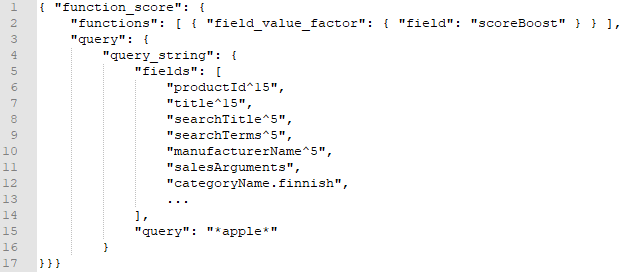
\includegraphics[width=\textwidth]{img/current-query.png}
    \caption{Current query used by the search application.}
    \label{fig:current-query}
\end{figure}


\section{Updating the search ranking scores}


The current search application ranks the results with a value from a field called \emph{scoreBoost},
shown in Figure \ref{fig:current-query}. 
The field is precalculated and updated to the persistent storage, and it
is indexed with the document at the same time as other data.
Thus, by using a precalculated field to rank the search results, the calculation necessary by the
search engine lessens.
Furthermore, there is no need to create a complicated ranking algorithm that the query uses
to extract values from multiple fields to calculate the score for the document.


As shown in Figure \ref{fig:current-solution}, the process behind updating the 
score boosts field to the persistent storage is a manual process.
The process of updating the score boosts is done manually by different individuals for four different websites.
The boosts are calculated by using an Excel file, which has been created to allow boosting based on 
various parameters, including margin, stock levels, and sales, in addition to allowing
different boosts based on category and brand of the product.


The process has been developed to keep boosting consistent across the different categories 
\cite{searchSurvey}.
The different parameters have been chosen based on empirical tests and  
expertise of the sales representatives across the categories \cite{searchSurvey}.
The knowledge about the category has been a relevant part when the process was created
since different parameters might vary across categories \cite{searchSurvey}.
For instance, the importance of a stock level might differ between a product that is 
continuously in stock and a product that must be ordered when a customer places an order
\cite{searchSurvey}.


Since there are tens of thousands of products active in each of the websites, the usage of a manual
process can be quite costly. 
However, not all products require to be separately boosted.
Some might just receive the boost based on their category or brand. 
The products that are in an upcoming campaign or are advertised may need special attention
\cite{searchSurvey}.
For an expert user, the process takes anywhere from 30 minutes to two hours to complete \cite{searchSurvey}.
Since the process is done by multiple individuals across the organization, the total
cost in person-hours can be hard to measure.


The benefits of using a manual process are that detailed
boosts can be achieved for specific situations, for instance, product campaigns \cite{relevantSearch}.
While the creation of specific boosts for a set of products takes time, it can be beneficial
to modify a specific boost for a product, if the parameters did not reflect the need well
\cite{searchSurvey}.


For instance, changing a boost to better match a query has been to introduce
an additional boost for iPads and Macbooks to better match the search query ``apple``.
While both are Apple products, neither mentions the word ``apple`` in the title and
iPhones do, the top of the results consist of entirely of IPhones, 
due to the high field-specific boost shown in Figure \ref{fig:current-query}.
Therefore, a need for boosting iPads and Macbooks was necessary and could be achieved with
an understanding of the domain and the manual process. \cite{searchSurvey}


